\section{Intelligence Artificielle et Industrie 4.0}\label{chap3:ia_industrie40}

\subsection{Qu'est-ce que l'Intelligence Artificielle?}

L'Intelligence Artificielle (IA) constitue un domaine fondamental de l'informatique moderne, visant à développer des systèmes capables d'effectuer des tâches requérant traditionnellement l'intelligence humaine. \cite{russell2010artificial} définissent l'IA comme \textit{"l'étude et la conception d'agents intelligents capables de percevoir leur environnement et de prendre des actions maximisant leurs chances de succès"}.

\subsubsection{Définitions et concepts fondamentaux}

L'Intelligence Artificielle englobe plusieurs paradigmes et approches complémentaires :

\begin{itemize}
    \item \textbf{Intelligence Artificielle symbolique} : Approche basée sur la manipulation de symboles et de règles logiques, dominante dans les années 1950-1980
    \item \textbf{Machine Learning (Apprentissage Automatique)} : Capacité des systèmes à apprendre à partir de données sans être explicitement programmés \cite{mitchell1997machine}
    \item \textbf{Deep Learning (Apprentissage Profond)} : Sous-domaine du ML utilisant des réseaux de neurones artificiels profonds pour modéliser des abstractions complexes
    \item \textbf{IA symbolique vs connexionniste} : Opposition historique entre approches basées sur la logique et celles basées sur les réseaux de neurones
\end{itemize}



\subsubsection{Paradigmes d'apprentissage en Machine Learning}

Le Machine Learning, cœur de l'IA moderne, se décline en plusieurs paradigmes d'apprentissage :

\begin{figure}[H]
\centering
\begin{tikzpicture}[
    node distance=2cm,
    box/.style={rectangle, draw, fill=blue!15, text width=3.5cm, text centered, rounded corners, minimum height=1.2cm, font=\small},
    arrow/.style={->, >=stealth, thick}
]

\node[box, fill=green!20] (ml) at (0,0) {\textbf{Machine Learning}};

\node[box] (supervised) at (-4,-2.5) {\textbf{Apprentissage\\Supervisé}};
\node[box] (unsupervised) at (0,-2.5) {\textbf{Apprentissage\\Non-Supervisé}};
\node[box] (reinforcement) at (4,-2.5) {\textbf{Apprentissage\\par Renforcement}};

\draw[arrow] (ml) -- (supervised);
\draw[arrow] (ml) -- (unsupervised);
\draw[arrow] (ml) -- (reinforcement);

\node[below=0.3cm of supervised, font=\footnotesize, text width=3.5cm, align=center] {
    Données étiquetées\\
    Classification, Régression
};

\node[below=0.3cm of unsupervised, font=\footnotesize, text width=3.5cm, align=center] {
    Données non étiquetées\\
    Clustering, Réduction
};

\node[below=0.3cm of reinforcement, font=\footnotesize, text width=3.5cm, align=center] {
    Récompenses/Pénalités\\
    Jeux, Robotique
};

\end{tikzpicture}
\caption{Paradigmes d'apprentissage en Machine Learning}
\label{fig:ml_paradigms}
\end{figure}

\textbf{Apprentissage Supervisé :}
\begin{itemize}
    \item Données d'entraînement étiquetées (paires entrée-sortie)
    \item Objectif : Apprendre une fonction de mapping $f: X \rightarrow Y$
    \item Applications : Classification (spam/non-spam), Régression (prédiction de prix)
    \item Algorithmes : Régression linéaire, SVM, Random Forest, XGBoost, Réseaux de neurones
\end{itemize}

\textbf{Apprentissage Non-Supervisé :}
\begin{itemize}
    \item Données sans étiquettes
    \item Objectif : Découvrir des structures cachées dans les données
    \item Applications : Segmentation clients, Détection d'anomalies, Réduction de dimensionnalité
    \item Algorithmes : K-means, DBSCAN, PCA, Autoencoders
\end{itemize}

\textbf{Apprentissage par Renforcement :}
\begin{itemize}
    \item Agent apprenant par interaction avec un environnement
    \item Objectif : Maximiser une récompense cumulative
    \item Applications : Jeux (AlphaGo), Robotique, Véhicules autonomes
    \item Algorithmes : Q-Learning, Deep Q-Networks (DQN), Policy Gradients
\end{itemize}

\subsection{L'Industrie 4.0 et la Transformation Digitale}

\subsubsection{Définition de l'Industrie 4.0}

L'Industrie 4.0, également appelée \textit{Quatrième Révolution Industrielle}, désigne la transformation digitale profonde des processus de fabrication et de production industrielle. Le terme a été introduit en 2011 lors du salon de Hanovre en Allemagne \cite{kagermann2013recommendations} et représente l'intégration des technologies numériques avancées dans l'ensemble de la chaîne de valeur industrielle.

L'Industrie 4.0 se caractérise par la convergence des technologies physiques, numériques et biologiques, créant des systèmes cyber-physiques (CPS) interconnectés capables de décisions autonomes et d'optimisation des processus de production en temps réel \cite{schwab2017fourth}.

\subsubsection{Les quatre révolutions industrielles}

L'histoire industrielle se divise en quatre révolutions majeures, chacune caractérisée par une innovation technologique disruptive :

\begin{figure}[H]
\centering
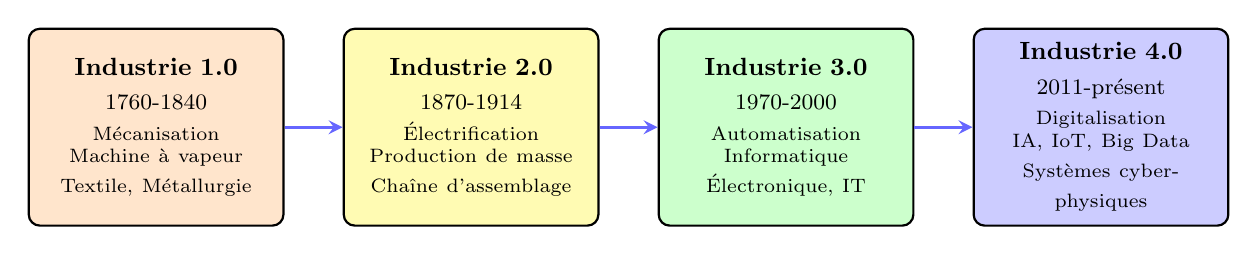
\begin{tikzpicture}[
    node distance=1.5cm,
    revolution/.style={rectangle, draw, thick, text width=3cm, text centered, rounded corners, minimum height=2.5cm, font=\small},
    arrow/.style={->, >=stealth, very thick, blue!60}
]

\node[revolution, fill=orange!20] (rev1) at (0,0) {
    \textbf{Industrie 1.0}\\[3pt]
    \footnotesize 1760-1840\\[3pt]
    \scriptsize Mécanisation\\
    Machine à vapeur\\
    Textile, Métallurgie
};

\node[revolution, fill=yellow!30] (rev2) at (4,0) {
    \textbf{Industrie 2.0}\\[3pt]
    \footnotesize 1870-1914\\[3pt]
    \scriptsize Électrification\\
    Production de masse\\
    Chaîne d'assemblage
};

\node[revolution, fill=green!20] (rev3) at (8,0) {
    \textbf{Industrie 3.0}\\[3pt]
    \footnotesize 1970-2000\\[3pt]
    \scriptsize Automatisation\\
    Informatique\\
    Électronique, IT
};

\node[revolution, fill=blue!20] (rev4) at (12,0) {
    \textbf{Industrie 4.0}\\[3pt]
    \footnotesize 2011-présent\\[3pt]
    \scriptsize Digitalisation\\
    IA, IoT, Big Data\\
    Systèmes cyber-physiques
};

\draw[arrow] (rev1) -- (rev2);
\draw[arrow] (rev2) -- (rev3);
\draw[arrow] (rev3) -- (rev4);

\end{tikzpicture}
\caption{Les quatre révolutions industrielles}
\label{fig:industrial_revolutions}
\end{figure}

\textbf{Industrie 1.0 (1760-1840) - Mécanisation}
\begin{itemize}
    \item \textbf{Innovation clé} : Machine à vapeur (James Watt, 1769)
    \item \textbf{Impact} : Remplacement de la force humaine/animale par la force mécanique
    \item \textbf{Secteurs} : Textile, métallurgie, transport ferroviaire
    \item \textbf{Gains} : Productivité multipliée par 10-20
\end{itemize}

\textbf{Industrie 2.0 (1870-1914) - Électrification et Production de Masse}
\begin{itemize}
    \item \textbf{Innovation clé} : Électricité, moteur à combustion interne
    \item \textbf{Impact} : Production de masse, standardisation, division du travail
    \item \textbf{Symbole} : Chaîne d'assemblage de Ford (1913)
    \item \textbf{Gains} : Réduction coûts de 60-70\%, démocratisation des produits
\end{itemize}

\textbf{Industrie 3.0 (1970-2000) - Automatisation et Informatisation}
\begin{itemize}
    \item \textbf{Innovation clé} : Ordinateurs, automates programmables (PLC), robots
    \item \textbf{Impact} : Automatisation des tâches répétitives, contrôle numérique
    \item \textbf{Technologies} : ERP, MES, SCADA, CAO/FAO
    \item \textbf{Gains} : Flexibilité +40\%, qualité +30\%, réduction main d'œuvre
\end{itemize}

\textbf{Industrie 4.0 (2011-présent) - Digitalisation et Intelligence}
\begin{itemize}
    \item \textbf{Innovation clé} : IA, IoT, Big Data, Cloud, Cyber-sécurité
    \item \textbf{Impact} : Systèmes autonomes, décisions en temps réel, personnalisation de masse
    \item \textbf{Paradigme} : Usine intelligente (Smart Factory), jumeau numérique (Digital Twin)
    \item \textbf{Gains attendus} : Productivité +30\%, flexibilité +50\%, time-to-market -40\%
\end{itemize}

\subsubsection{Les piliers technologiques de l'Industrie 4.0}

L'Industrie 4.0 repose sur neuf piliers technologiques interconnectés \cite{rüßmann2015industry} :

\begin{figure}[H]
\centering
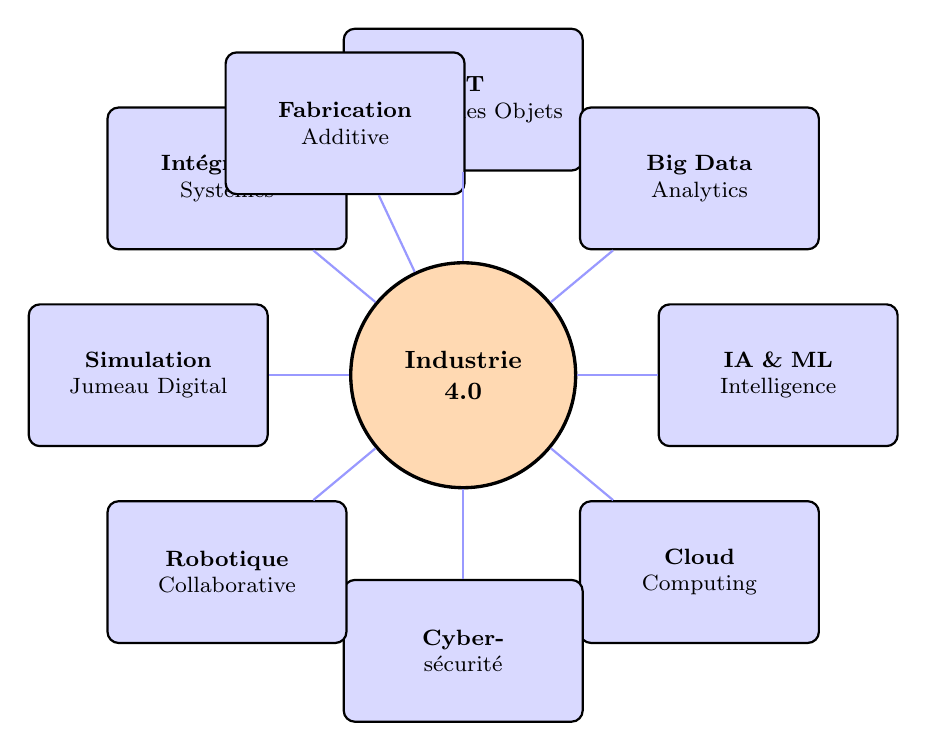
\begin{tikzpicture}[
    node distance=0.3cm,
    pillar/.style={rectangle, draw, thick, fill=blue!15, text width=2.8cm, text centered, rounded corners, minimum height=1.8cm, font=\footnotesize},
    center/.style={circle, draw, very thick, fill=orange!30, text width=2.5cm, text centered, font=\small\bfseries}
]

% Centre
\node[center] (center) at (0,0) {Industrie\\4.0};

% Piliers autour (disposition circulaire)
\node[pillar] (iot) at (0,3.5) {\textbf{IoT}\\Internet des Objets};
\node[pillar] (bigdata) at (3,2.5) {\textbf{Big Data}\\Analytics};
\node[pillar] (ai) at (4,0) {\textbf{IA \& ML}\\Intelligence};
\node[pillar] (cloud) at (3,-2.5) {\textbf{Cloud}\\Computing};
\node[pillar] (cyber) at (0,-3.5) {\textbf{Cyber-}\\sécurité};
\node[pillar] (robot) at (-3,-2.5) {\textbf{Robotique}\\Collaborative};
\node[pillar] (simulation) at (-4,0) {\textbf{Simulation}\\Jumeau Digital};
\node[pillar] (integration) at (-3,2.5) {\textbf{Intégration}\\Systèmes};
\node[pillar] (additive) at (-1.5,3.2) {\textbf{Fabrication}\\Additive};

% Connexions
\foreach \pillar in {iot, bigdata, ai, cloud, cyber, robot, simulation, integration, additive}
    \draw[thick, blue!40] (center) -- (\pillar);

\end{tikzpicture}
\caption{Les neuf piliers technologiques de l'Industrie 4.0}
\label{fig:industry40_pillars}
\end{figure}

\textbf{1. Internet des Objets (IoT - Internet of Things)}

Réseau de capteurs et d'actionneurs connectés collectant et échangeant des données en temps réel.

\begin{itemize}
    \item \textbf{Technologies} : Capteurs RFID, NFC, Bluetooth, LoRa, 5G
    \item \textbf{Applications} : Suivi des actifs, monitoring machines, traçabilité produits
    \item \textbf{Impact} : Visibilité temps réel, maintenance prédictive, optimisation énergétique
    \item \textbf{Chiffres} : 75 milliards d'objets connectés prévus en 2025 (IDC)
\end{itemize}

\textbf{2. Big Data et Analytics}

Capacité à collecter, stocker et analyser des volumes massifs de données hétérogènes.

\begin{itemize}
    \item \textbf{Caractéristiques} : Volume (pétaoctets), Vélocité (temps réel), Variété (structuré/non-structuré)
    \item \textbf{Technologies} : Hadoop, Spark, NoSQL, Data Lakes
    \item \textbf{Applications} : Analyse prédictive, détection d'anomalies, optimisation processus
    \item \textbf{Impact} : Décisions data-driven, amélioration continue, innovation produits
\end{itemize}

\textbf{3. Intelligence Artificielle et Machine Learning}

Systèmes capables d'apprendre, de raisonner et de prendre des décisions autonomes.

\begin{itemize}
    \item \textbf{Techniques} : Apprentissage supervisé, non-supervisé, par renforcement, Deep Learning
    \item \textbf{Applications} : Prédiction demande, contrôle qualité visuel, optimisation planning
    \item \textbf{Impact} : Automatisation décisions complexes, personnalisation, efficacité +25-40\%
    \item \textbf{Investissements} : 500 milliards USD prévus en 2024 (IDC)
\end{itemize}

\textbf{4. Cloud Computing}

Infrastructure informatique distribuée accessible à la demande via Internet.

\begin{itemize}
    \item \textbf{Modèles} : IaaS, PaaS, SaaS, Edge Computing
    \item \textbf{Avantages} : Scalabilité, flexibilité, réduction coûts IT, accessibilité
    \item \textbf{Applications} : ERP cloud, MES cloud, collaboration, backup
    \item \textbf{Adoption} : 94\% des entreprises utilisent le cloud (Flexera 2023)
\end{itemize}

\textbf{5. Cyber-sécurité}

Protection des systèmes industriels contre les cyberattaques et les intrusions.

\begin{itemize}
    \item \textbf{Enjeux} : Interconnexion accrue = surface d'attaque élargie
    \item \textbf{Technologies} : Firewalls industriels, détection d'intrusion, chiffrement
    \item \textbf{Standards} : IEC 62443, ISO 27001, NIST Cybersecurity Framework
    \item \textbf{Coût} : Cyberattaques coûtent 6 trillions USD/an globalement (Cybersecurity Ventures)
\end{itemize}

\textbf{6. Robotique Collaborative (Cobots)}

Robots conçus pour travailler en collaboration directe avec les humains.

\begin{itemize}
    \item \textbf{Caractéristiques} : Sécurité intrinsèque, facilité de programmation, flexibilité
    \item \textbf{Applications} : Assemblage, pick-and-place, contrôle qualité, emballage
    \item \textbf{Impact} : Productivité +30\%, ergonomie améliorée, réduction TMS
    \item \textbf{Marché} : Croissance 40\% CAGR 2020-2027 (MarketsandMarkets)
\end{itemize}

\textbf{7. Simulation et Jumeau Numérique (Digital Twin)}

Réplique virtuelle d'un système physique permettant simulation et optimisation.

\begin{itemize}
    \item \textbf{Concept} : Modèle numérique synchronisé avec le système réel via IoT
    \item \textbf{Applications} : Test de scénarios, optimisation paramètres, formation, maintenance
    \item \textbf{Impact} : Réduction time-to-market -50\%, coûts R\&D -30\%, qualité +25\%
    \item \textbf{Adoption} : 75\% des grandes entreprises industrielles en 2025 (Gartner)
\end{itemize}

\textbf{8. Intégration Horizontale et Verticale}

Interconnexion des systèmes à tous les niveaux de l'entreprise et de la chaîne de valeur.

\begin{itemize}
    \item \textbf{Verticale} : ERP $\leftrightarrow$ MES $\leftrightarrow$ SCADA $\leftrightarrow$ Capteurs (pyramide CIM)
    \item \textbf{Horizontale} : Intégration fournisseurs-production-clients (Supply Chain)
    \item \textbf{Technologies} : API, middleware, bus de données, standards (OPC UA)
    \item \textbf{Impact} : Visibilité end-to-end, agilité, réduction silos
\end{itemize}

\textbf{9. Fabrication Additive (Impression 3D)}

Technologies de fabrication par ajout de matière couche par couche.

\begin{itemize}
    \item \textbf{Procédés} : FDM, SLA, SLS, DMLS (métaux)
    \item \textbf{Applications} : Prototypage rapide, pièces de rechange, personnalisation
    \item \textbf{Impact} : Réduction délais -70\%, complexité géométrique, production décentralisée
    \item \textbf{Marché} : 50 milliards USD en 2028 (Wohlers Report)
\end{itemize}







